% Coordinates copied from the CSV fields stated beside each series.
\begin{figure}[p]
\centering
\resizebox{\textwidth}{!}{%
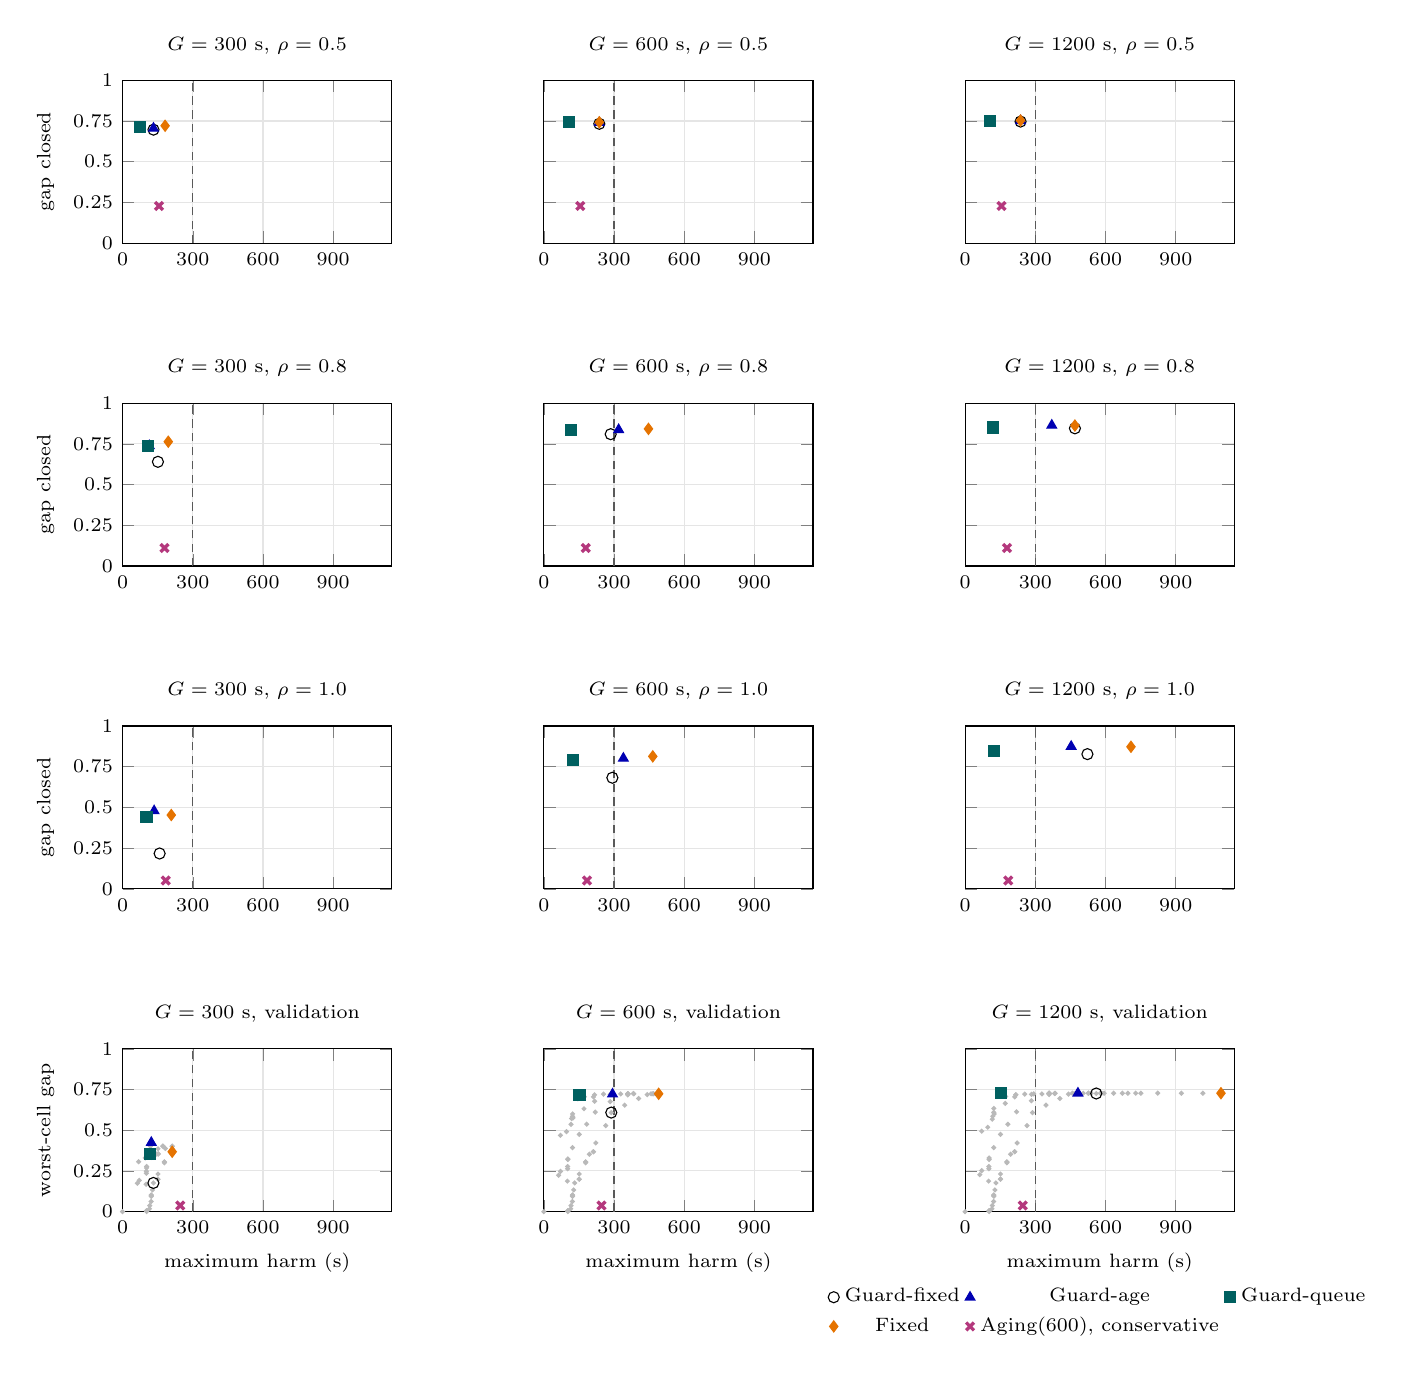
\begin{tikzpicture}
\pgfplotsset{tradeaxis/.style={width=5cm,height=3.65cm,
 xmin=0,xmax=1150,ymin=0,ymax=1,xtick={0,300,600,900},
 ytick={0,0.25,0.5,0.75,1},grid=major,grid style={black!10},
 tick label style={font=\scriptsize},label style={font=\scriptsize},
 title style={font=\scriptsize},mark size=2pt}}
\begin{axis}[tradeaxis,name=cell00,at={(0.0cm,0.0cm)},title={$G=300$ s, $\rho=0.5$},ylabel={gap closed}]
\addplot[black!65,densely dashed,no marks,forget plot] coordinates {(300,0) (300,1)};
% Source: outputs/selection_v4/selected_parameters.csv, G=600, harm_limit_s=300.
\addplot[only marks,mark=o,black] coordinates {(132.113597,0.696832)};
% Source: outputs/dev_tables/main_table.csv, level=0, policy=Guard-fixed(300), harm_s/gap_closed.
\addplot[only marks,mark=triangle*,blue!70!black] coordinates {(132.113597,0.705158)};
% Source: outputs/dev_tables/main_table.csv, level=0, policy=Guard-age(300), harm_s/gap_closed.
\addplot[only marks,mark=square*,teal!75!black] coordinates {(75.095370,0.713665)};
% Source: outputs/dev_tables/main_table.csv, level=0, policy=Guard-queue(300), harm_s/gap_closed.
\addplot[only marks,mark=diamond*,orange!90!black] coordinates {(181.775646,0.720709)};
% Source: outputs/dev_tables/main_table.csv, level=0, policy=Fixed(300), harm_s/gap_closed.
\addplot[only marks,mark=x,very thick,magenta!70!black] coordinates {(155.750511,0.228444)};
% Source: outputs/dev_visibility/visibility_comparison.csv, level=0, policy=Aging(600), harm_s/gap_closed.
\end{axis}
\begin{axis}[tradeaxis,name=cell01,at={(5.35cm,0.0cm)},title={$G=600$ s, $\rho=0.5$},yticklabels={}]
\addplot[black!65,densely dashed,no marks,forget plot] coordinates {(300,0) (300,1)};
% Source: outputs/selection_v4/selected_parameters.csv, G=600, harm_limit_s=300.
\addplot[only marks,mark=o,black] coordinates {(237.038507,0.732794)};
% Source: outputs/dev_tables/main_table.csv, level=0, policy=Guard-fixed(600), harm_s/gap_closed.
\addplot[only marks,mark=triangle*,blue!70!black] coordinates {(237.038507,0.739757)};
% Source: outputs/dev_tables/main_table.csv, level=0, policy=Guard-age(600), harm_s/gap_closed.
\addplot[only marks,mark=square*,teal!75!black] coordinates {(105.996310,0.744373)};
% Source: outputs/dev_tables/main_table.csv, level=0, policy=Guard-queue(600), harm_s/gap_closed.
\addplot[only marks,mark=diamond*,orange!90!black] coordinates {(237.038507,0.742355)};
% Source: outputs/dev_tables/main_table.csv, level=0, policy=Fixed(600), harm_s/gap_closed.
\addplot[only marks,mark=x,very thick,magenta!70!black] coordinates {(155.750511,0.228444)};
% Source: outputs/dev_visibility/visibility_comparison.csv, level=0, policy=Aging(600), harm_s/gap_closed.
\end{axis}
\begin{axis}[tradeaxis,name=cell02,at={(10.7cm,0.0cm)},title={$G=1200$ s, $\rho=0.5$},yticklabels={}]
\addplot[black!65,densely dashed,no marks,forget plot] coordinates {(300,0) (300,1)};
% Source: outputs/selection_v4/selected_parameters.csv, G=600, harm_limit_s=300.
\addplot[only marks,mark=o,black] coordinates {(237.038507,0.746565)};
% Source: outputs/dev_tables/main_table.csv, level=0, policy=Guard-fixed(1200), harm_s/gap_closed.
\addplot[only marks,mark=triangle*,blue!70!black] coordinates {(237.038507,0.751273)};
% Source: outputs/dev_tables/main_table.csv, level=0, policy=Guard-age(1200), harm_s/gap_closed.
\addplot[only marks,mark=square*,teal!75!black] coordinates {(105.996310,0.749753)};
% Source: outputs/dev_tables/main_table.csv, level=0, policy=Guard-queue(1200), harm_s/gap_closed.
\addplot[only marks,mark=diamond*,orange!90!black] coordinates {(237.038507,0.753101)};
% Source: outputs/dev_tables/main_table.csv, level=0, policy=Fixed(1200), harm_s/gap_closed.
\addplot[only marks,mark=x,very thick,magenta!70!black] coordinates {(155.750511,0.228444)};
% Source: outputs/dev_visibility/visibility_comparison.csv, level=0, policy=Aging(600), harm_s/gap_closed.
\end{axis}
\begin{axis}[tradeaxis,name=cell10,at={(0.0cm,-4.1cm)},title={$G=300$ s, $\rho=0.8$},ylabel={gap closed}]
\addplot[black!65,densely dashed,no marks,forget plot] coordinates {(300,0) (300,1)};
% Source: outputs/selection_v4/selected_parameters.csv, G=600, harm_limit_s=300.
\addplot[only marks,mark=o,black] coordinates {(151.108458,0.639557)};
% Source: outputs/dev_tables/main_table.csv, level=1, policy=Guard-fixed(300), harm_s/gap_closed.
\addplot[only marks,mark=triangle*,blue!70!black] coordinates {(114.105582,0.738150)};
% Source: outputs/dev_tables/main_table.csv, level=1, policy=Guard-age(300), harm_s/gap_closed.
\addplot[only marks,mark=square*,teal!75!black] coordinates {(109.500007,0.735903)};
% Source: outputs/dev_tables/main_table.csv, level=1, policy=Guard-queue(300), harm_s/gap_closed.
\addplot[only marks,mark=diamond*,orange!90!black] coordinates {(195.368590,0.763038)};
% Source: outputs/dev_tables/main_table.csv, level=1, policy=Fixed(300), harm_s/gap_closed.
\addplot[only marks,mark=x,very thick,magenta!70!black] coordinates {(179.091488,0.110733)};
% Source: outputs/dev_visibility/visibility_comparison.csv, level=1, policy=Aging(600), harm_s/gap_closed.
\end{axis}
\begin{axis}[tradeaxis,name=cell11,at={(5.35cm,-4.1cm)},title={$G=600$ s, $\rho=0.8$},yticklabels={}]
\addplot[black!65,densely dashed,no marks,forget plot] coordinates {(300,0) (300,1)};
% Source: outputs/selection_v4/selected_parameters.csv, G=600, harm_limit_s=300.
\addplot[only marks,mark=o,black] coordinates {(285.684511,0.809203)};
% Source: outputs/dev_tables/main_table.csv, level=1, policy=Guard-fixed(600), harm_s/gap_closed.
\addplot[only marks,mark=triangle*,blue!70!black] coordinates {(319.640469,0.836835)};
% Source: outputs/dev_tables/main_table.csv, level=1, policy=Guard-age(600), harm_s/gap_closed.
\addplot[only marks,mark=square*,teal!75!black] coordinates {(117.695233,0.834292)};
% Source: outputs/dev_tables/main_table.csv, level=1, policy=Guard-queue(600), harm_s/gap_closed.
\addplot[only marks,mark=diamond*,orange!90!black] coordinates {(447.100987,0.841959)};
% Source: outputs/dev_tables/main_table.csv, level=1, policy=Fixed(600), harm_s/gap_closed.
\addplot[only marks,mark=x,very thick,magenta!70!black] coordinates {(179.091488,0.110733)};
% Source: outputs/dev_visibility/visibility_comparison.csv, level=1, policy=Aging(600), harm_s/gap_closed.
\end{axis}
\begin{axis}[tradeaxis,name=cell12,at={(10.7cm,-4.1cm)},title={$G=1200$ s, $\rho=0.8$},yticklabels={}]
\addplot[black!65,densely dashed,no marks,forget plot] coordinates {(300,0) (300,1)};
% Source: outputs/selection_v4/selected_parameters.csv, G=600, harm_limit_s=300.
\addplot[only marks,mark=o,black] coordinates {(469.226797,0.845169)};
% Source: outputs/dev_tables/main_table.csv, level=1, policy=Guard-fixed(1200), harm_s/gap_closed.
\addplot[only marks,mark=triangle*,blue!70!black] coordinates {(370.455235,0.863896)};
% Source: outputs/dev_tables/main_table.csv, level=1, policy=Guard-age(1200), harm_s/gap_closed.
\addplot[only marks,mark=square*,teal!75!black] coordinates {(117.695233,0.850311)};
% Source: outputs/dev_tables/main_table.csv, level=1, policy=Guard-queue(1200), harm_s/gap_closed.
\addplot[only marks,mark=diamond*,orange!90!black] coordinates {(469.226797,0.862203)};
% Source: outputs/dev_tables/main_table.csv, level=1, policy=Fixed(1200), harm_s/gap_closed.
\addplot[only marks,mark=x,very thick,magenta!70!black] coordinates {(179.091488,0.110733)};
% Source: outputs/dev_visibility/visibility_comparison.csv, level=1, policy=Aging(600), harm_s/gap_closed.
\end{axis}
\begin{axis}[tradeaxis,name=cell20,at={(0.0cm,-8.2cm)},title={$G=300$ s, $\rho=1.0$},ylabel={gap closed}]
\addplot[black!65,densely dashed,no marks,forget plot] coordinates {(300,0) (300,1)};
% Source: outputs/selection_v4/selected_parameters.csv, G=600, harm_limit_s=300.
\addplot[only marks,mark=o,black] coordinates {(158.368944,0.216879)};
% Source: outputs/dev_tables/main_table.csv, level=2, policy=Guard-fixed(300), harm_s/gap_closed.
\addplot[only marks,mark=triangle*,blue!70!black] coordinates {(134.822787,0.478471)};
% Source: outputs/dev_tables/main_table.csv, level=2, policy=Guard-age(300), harm_s/gap_closed.
\addplot[only marks,mark=square*,teal!75!black] coordinates {(102.234025,0.442394)};
% Source: outputs/dev_tables/main_table.csv, level=2, policy=Guard-queue(300), harm_s/gap_closed.
\addplot[only marks,mark=diamond*,orange!90!black] coordinates {(208.168830,0.453176)};
% Source: outputs/dev_tables/main_table.csv, level=2, policy=Fixed(300), harm_s/gap_closed.
\addplot[only marks,mark=x,very thick,magenta!70!black] coordinates {(184.681683,0.051198)};
% Source: outputs/dev_visibility/visibility_comparison.csv, level=2, policy=Aging(600), harm_s/gap_closed.
\end{axis}
\begin{axis}[tradeaxis,name=cell21,at={(5.35cm,-8.2cm)},title={$G=600$ s, $\rho=1.0$},yticklabels={}]
\addplot[black!65,densely dashed,no marks,forget plot] coordinates {(300,0) (300,1)};
% Source: outputs/selection_v4/selected_parameters.csv, G=600, harm_limit_s=300.
\addplot[only marks,mark=o,black] coordinates {(292.893082,0.682027)};
% Source: outputs/dev_tables/main_table.csv, level=2, policy=Guard-fixed(600), harm_s/gap_closed.
\addplot[only marks,mark=triangle*,blue!70!black] coordinates {(339.882000,0.801314)};
% Source: outputs/dev_tables/main_table.csv, level=2, policy=Guard-age(600), harm_s/gap_closed.
\addplot[only marks,mark=square*,teal!75!black] coordinates {(123.391351,0.793065)};
% Source: outputs/dev_tables/main_table.csv, level=2, policy=Guard-queue(600), harm_s/gap_closed.
\addplot[only marks,mark=diamond*,orange!90!black] coordinates {(465.528424,0.813125)};
% Source: outputs/dev_tables/main_table.csv, level=2, policy=Fixed(600), harm_s/gap_closed.
\addplot[only marks,mark=x,very thick,magenta!70!black] coordinates {(184.681683,0.051198)};
% Source: outputs/dev_visibility/visibility_comparison.csv, level=2, policy=Aging(600), harm_s/gap_closed.
\end{axis}
\begin{axis}[tradeaxis,name=cell22,at={(10.7cm,-8.2cm)},title={$G=1200$ s, $\rho=1.0$},yticklabels={}]
\addplot[black!65,densely dashed,no marks,forget plot] coordinates {(300,0) (300,1)};
% Source: outputs/selection_v4/selected_parameters.csv, G=600, harm_limit_s=300.
\addplot[only marks,mark=o,black] coordinates {(522.663563,0.826977)};
% Source: outputs/dev_tables/main_table.csv, level=2, policy=Guard-fixed(1200), harm_s/gap_closed.
\addplot[only marks,mark=triangle*,blue!70!black] coordinates {(453.326274,0.874075)};
% Source: outputs/dev_tables/main_table.csv, level=2, policy=Guard-age(1200), harm_s/gap_closed.
\addplot[only marks,mark=square*,teal!75!black] coordinates {(123.391351,0.844280)};
% Source: outputs/dev_tables/main_table.csv, level=2, policy=Guard-queue(1200), harm_s/gap_closed.
\addplot[only marks,mark=diamond*,orange!90!black] coordinates {(708.755315,0.872237)};
% Source: outputs/dev_tables/main_table.csv, level=2, policy=Fixed(1200), harm_s/gap_closed.
\addplot[only marks,mark=x,very thick,magenta!70!black] coordinates {(184.681683,0.051198)};
% Source: outputs/dev_visibility/visibility_comparison.csv, level=2, policy=Aging(600), harm_s/gap_closed.
\end{axis}
\begin{axis}[tradeaxis,name=cell30,at={(0.0cm,-12.299999999999999cm)},title={$G=300$ s, validation},ylabel={worst-cell gap},xlabel={maximum harm (s)}]
\addplot[black!65,densely dashed,no marks,forget plot] coordinates {(300,0) (300,1)};
% Source: outputs/selection_v4/selected_parameters.csv, G=600, harm_limit_s=300.
\addplot[only marks,mark=*,mark size=0.7pt,gray!55,forget plot] coordinates {(122.755698,0.424289) (124.486727,0.416017) (122.740501,0.409477) (171.631136,0.403032) (212.065268,0.402958) (173.432647,0.401495) (118.668152,0.401358) (212.065268,0.400341) (182.959608,0.388243) (151.328698,0.386288) (212.065268,0.382721) (212.065268,0.375584) (212.065268,0.375154) (212.065268,0.370421) (212.065268,0.370045) (212.065268,0.370028) (212.065268,0.369773) (212.065268,0.368993) (212.065268,0.367911) (212.065268,0.367911) (212.065268,0.367911) (212.065268,0.367911) (212.065268,0.367911) (212.065268,0.367911) (212.065268,0.367911) (212.065268,0.367911) (212.065268,0.367911) (212.065268,0.367911) (212.065268,0.367911) (212.065268,0.367911) (212.065268,0.367911) (212.065268,0.367911) (212.065268,0.367911) (212.065268,0.367911) (212.065268,0.367911) (212.065268,0.367911) (212.065268,0.367911) (212.065268,0.367911) (212.065268,0.367911) (212.065268,0.367911) (212.065268,0.367911) (122.564115,0.333720) (178.891097,0.305259) (102.728126,0.277283) (101.644038,0.247694) (101.644038,0.235701) (151.176160,0.199383) (100.614810,0.168602) (122.564115,0.101841) (102.641448,0.005695) (0.000000,0.000000) (66.635225,-0.006938) (71.317912,-0.010291) (96.276594,-0.012546) (212.065268,0.367911) (178.891097,0.305259) (178.891097,0.300021) (151.328698,0.231224) (151.176160,0.199383) (131.802082,0.176325) (127.572451,0.133352) (122.564115,0.101841) (122.564115,0.094309) (122.158704,0.062245) (116.249557,0.037365) (115.042103,0.017902) (102.641448,0.005695) (102.641448,0.000386) (66.635225,-0.006938) (102.641448,-0.008509) (66.635225,-0.009444) (96.284759,-0.010129) (71.317912,-0.010291) (66.635225,-0.010313) (71.317912,-0.010453) (96.276594,-0.010688) (66.635225,-0.010827) (80.544101,-0.012472) (96.276594,-0.012546) (71.317912,-0.012791) (96.276594,-0.014005) (212.065268,0.370159) (212.065268,0.369222) (212.065268,0.368964) (212.065268,0.368550) (212.065268,0.367958) (212.065268,0.367911) (212.065268,0.367911) (212.065268,0.367911) (212.065268,0.367911) (116.249557,0.354832) (152.154055,0.354716) (151.665881,0.353887) (145.308175,0.353427) (96.847341,0.329525) (68.659387,0.306918) (102.641448,0.268386) (71.317912,0.192447) (63.109644,0.173796)};
% Source: outputs/selection_v4/selection_frontier.csv, promise_s=300, worst_harm_s/worst_gap_closed (all candidate rows).
\addplot[only marks,mark=o,black] coordinates {(131.802082,0.176325)};
% Source: outputs/selection_v4/selected_parameters.csv, family=fixed, promise_s=300.
\addplot[only marks,mark=triangle*,blue!70!black] coordinates {(122.755698,0.424289)};
% Source: outputs/selection_v4/selected_parameters.csv, family=capped, promise_s=300.
\addplot[only marks,mark=square*,teal!75!black] coordinates {(116.249557,0.354832)};
% Source: outputs/selection_v4/selected_parameters.csv, family=hybrid, promise_s=300.
\addplot[only marks,mark=diamond*,orange!90!black] coordinates {(212.065268,0.367911)};
% Source: outputs/selection_v4/selection_worst.csv, fixed/inf, promise_s=300.
\addplot[only marks,mark=x,very thick,magenta!70!black] coordinates {(246.359636,0.037527)};
% Source: outputs/selection_aging/selected_aging.csv, worst_harm_s/worst_gap_closed.
\end{axis}
\begin{axis}[tradeaxis,name=cell31,at={(5.35cm,-12.299999999999999cm)},title={$G=600$ s, validation},yticklabels={},xlabel={maximum harm (s)}]
\addplot[black!65,densely dashed,no marks,forget plot] coordinates {(300,0) (300,1)};
% Source: outputs/selection_v4/selected_parameters.csv, G=600, harm_limit_s=300.
\addplot[only marks,mark=*,mark size=0.7pt,gray!55,forget plot] coordinates {(382.544103,0.725544) (482.360035,0.723773) (482.360035,0.723773) (490.534049,0.723773) (490.534049,0.723773) (490.534049,0.723773) (482.163584,0.723773) (490.534049,0.723773) (490.534049,0.723773) (490.534049,0.723773) (490.534049,0.723773) (490.534049,0.723773) (490.534049,0.723773) (490.534049,0.723773) (490.534049,0.723773) (358.921846,0.723696) (482.360035,0.723325) (384.634906,0.723149) (358.921846,0.723142) (482.606574,0.723026) (328.403010,0.722855) (293.453790,0.721576) (254.958484,0.721385) (358.921846,0.721373) (283.589795,0.720267) (441.653011,0.718335) (216.809921,0.716930) (358.921846,0.716709) (173.432647,0.705608) (212.083511,0.704189) (216.809921,0.677888) (283.453074,0.675658) (171.631136,0.631730) (219.926614,0.610881) (122.755698,0.599837) (122.740501,0.585033) (124.486727,0.575706) (118.668152,0.571446) (182.959608,0.537136) (151.328698,0.474246) (122.564115,0.393579) (212.065268,0.367911) (102.728126,0.320504) (178.891097,0.305259) (101.644038,0.277130) (101.644038,0.263620) (151.176160,0.199383) (100.614810,0.187331) (122.564115,0.101841) (102.641448,0.005695) (0.000000,0.000000) (66.635225,-0.006938) (71.317912,-0.010291) (96.276594,-0.012546) (465.726735,0.724372) (490.534049,0.723773) (404.872507,0.694634) (345.441058,0.653912) (288.186805,0.608249) (264.673346,0.528176) (222.348080,0.422093) (212.065268,0.367911) (194.483690,0.352687) (178.891097,0.305259) (178.891097,0.300021) (151.328698,0.231224) (151.176160,0.199383) (131.802082,0.176325) (127.572451,0.133352) (122.564115,0.101841) (122.564115,0.094309) (122.158704,0.062245) (116.249557,0.037365) (115.042103,0.017902) (102.641448,0.005695) (102.641448,0.000386) (66.635225,-0.006938) (102.641448,-0.008509) (66.635225,-0.009444) (96.284759,-0.010129) (71.317912,-0.010291) (66.635225,-0.010313) (71.317912,-0.010453) (96.276594,-0.010688) (66.635225,-0.010827) (80.544101,-0.012472) (96.276594,-0.012546) (71.317912,-0.012791) (96.276594,-0.014005) (458.014105,0.723773) (358.921846,0.723773) (469.184788,0.723773) (482.360035,0.723773) (482.360035,0.723773) (482.360035,0.723773) (358.921846,0.723220) (358.921846,0.723189) (358.921846,0.722679) (152.154055,0.716287) (151.665881,0.699375) (145.308175,0.692937) (116.249557,0.536272) (96.847341,0.491557) (71.044501,0.468659) (102.641448,0.323748) (71.317912,0.247493) (63.109644,0.223238)};
% Source: outputs/selection_v4/selection_frontier.csv, promise_s=600, worst_harm_s/worst_gap_closed (all candidate rows).
\addplot[only marks,mark=o,black] coordinates {(288.186805,0.608249)};
% Source: outputs/selection_v4/selected_parameters.csv, family=fixed, promise_s=600.
\addplot[only marks,mark=triangle*,blue!70!black] coordinates {(293.453790,0.721576)};
% Source: outputs/selection_v4/selected_parameters.csv, family=capped, promise_s=600.
\addplot[only marks,mark=square*,teal!75!black] coordinates {(152.154055,0.716287)};
% Source: outputs/selection_v4/selected_parameters.csv, family=hybrid, promise_s=600.
\addplot[only marks,mark=diamond*,orange!90!black] coordinates {(490.534049,0.723773)};
% Source: outputs/selection_v4/selection_worst.csv, fixed/inf, promise_s=600.
\addplot[only marks,mark=x,very thick,magenta!70!black] coordinates {(246.359636,0.037527)};
% Source: outputs/selection_aging/selected_aging.csv, worst_harm_s/worst_gap_closed.
\end{axis}
\begin{axis}[tradeaxis,name=cell32,at={(10.7cm,-12.299999999999999cm)},title={$G=1200$ s, validation},yticklabels={},xlabel={maximum harm (s)},legend style={at={(0.5,-0.40)},anchor=north,legend columns=3,font=\scriptsize,draw=none}]
\addplot[black!65,densely dashed,no marks,forget plot] coordinates {(300,0) (300,1)};
% Source: outputs/selection_v4/selected_parameters.csv, G=600, harm_limit_s=300.
\addplot[only marks,mark=*,mark size=0.7pt,gray!55,forget plot] coordinates {(729.043192,0.727225) (526.907504,0.727225) (1016.146018,0.727225) (823.125753,0.727225) (1093.309521,0.727225) (482.163584,0.727225) (1093.309521,0.727225) (1093.309521,0.727225) (594.086778,0.727225) (1093.309521,0.727225) (1093.309521,0.727225) (695.460722,0.727225) (1093.309521,0.727225) (1093.309521,0.727225) (583.959065,0.726979) (384.634906,0.726750) (504.633396,0.726648) (358.921846,0.726273) (382.544103,0.725439) (358.921846,0.724968) (358.921846,0.723307) (293.453790,0.723220) (328.403010,0.722855) (254.958484,0.722137) (441.653011,0.721763) (283.589795,0.720267) (358.921846,0.718653) (216.809921,0.718258) (216.809921,0.717456) (173.432647,0.707399) (212.083511,0.704899) (283.453074,0.681206) (171.631136,0.665109) (122.755698,0.633595) (219.926614,0.613094) (122.740501,0.609656) (124.486727,0.599878) (118.668152,0.586456) (182.959608,0.536589) (151.328698,0.474467) (122.564115,0.393579) (212.065268,0.367911) (102.728126,0.320504) (178.891097,0.305259) (101.644038,0.277130) (101.644038,0.263620) (151.176160,0.199383) (100.614810,0.187331) (122.564115,0.101841) (102.641448,0.005695) (0.000000,0.000000) (66.635225,-0.006938) (71.317912,-0.010291) (96.276594,-0.012546) (634.849609,0.727225) (751.028293,0.727225) (924.041389,0.727225) (1093.309521,0.727225) (560.338925,0.725554) (465.726735,0.724372) (404.872507,0.694634) (345.441058,0.653912) (288.186805,0.608249) (264.673346,0.528176) (222.348080,0.422093) (212.065268,0.367911) (194.483690,0.352687) (178.891097,0.305259) (178.891097,0.300021) (151.328698,0.231224) (151.176160,0.199383) (131.802082,0.176325) (127.572451,0.133352) (122.564115,0.101841) (122.564115,0.094309) (122.158704,0.062245) (116.249557,0.037365) (115.042103,0.017902) (102.641448,0.005695) (102.641448,0.000386) (66.635225,-0.006938) (102.641448,-0.008509) (66.635225,-0.009444) (96.284759,-0.010129) (71.317912,-0.010291) (66.635225,-0.010313) (71.317912,-0.010453) (96.276594,-0.010688) (66.635225,-0.010827) (80.544101,-0.012472) (96.276594,-0.012546) (71.317912,-0.012791) (96.276594,-0.014005) (152.154055,0.727488) (145.308175,0.727428) (458.085089,0.727225) (358.921846,0.727225) (526.723892,0.727225) (538.334839,0.727225) (577.597193,0.727225) (672.258107,0.727225) (358.921846,0.726931) (358.921846,0.726885) (358.921846,0.724468) (151.665881,0.721121) (116.249557,0.567430) (96.847341,0.518252) (71.044501,0.494108) (102.641448,0.329446) (71.317912,0.252063) (63.109644,0.227268)};
% Source: outputs/selection_v4/selection_frontier.csv, promise_s=1200, worst_harm_s/worst_gap_closed (all candidate rows).
\addplot[only marks,mark=o,black] coordinates {(560.338925,0.725554)};
% Source: outputs/selection_v4/selected_parameters.csv, family=fixed, promise_s=1200.
\addlegendentry{Guard-fixed}
\addplot[only marks,mark=triangle*,blue!70!black] coordinates {(482.163584,0.727225)};
% Source: outputs/selection_v4/selected_parameters.csv, family=capped, promise_s=1200.
\addlegendentry{Guard-age}
\addplot[only marks,mark=square*,teal!75!black] coordinates {(152.154055,0.727488)};
% Source: outputs/selection_v4/selected_parameters.csv, family=hybrid, promise_s=1200.
\addlegendentry{Guard-queue}
\addplot[only marks,mark=diamond*,orange!90!black] coordinates {(1093.309521,0.727225)};
% Source: outputs/selection_v4/selection_worst.csv, fixed/inf, promise_s=1200.
\addlegendentry{Fixed}
\addplot[only marks,mark=x,very thick,magenta!70!black] coordinates {(246.359636,0.037527)};
% Source: outputs/selection_aging/selected_aging.csv, worst_harm_s/worst_gap_closed.
\addlegendentry{Aging(600), conservative}
\end{axis}
\end{tikzpicture}}
\caption{Gap--harm trade-offs for every selected budget shape and Fixed($G$), at each
promise and load (upper rows); validation candidates and per-family selections
(bottom row). A joint winner coincides with its selected family point. The dashed
line is the \devnum{300} s validation limit for $G=\devnum{600}$ s; it is shown in
every panel as a common reference, not as the constraint for every promise.
The other promise-specific limits follow harm $\le G/2$.
All budget-family points use original scores. The magenta point is the only selected
aging comparator, Aging(600), with conservative scores and no proved guarantee;
it is repeated across promise panels for orientation, not retuned at other promises.
Cross-protocol points do not establish Pareto dominance. Maxima have no population
interval; gap intervals for the selected rows are reported in the tables.}
% Sources: outputs/selection_v4/selected_parameters.csv (harm_limit_s=300 for G=600);
% all plotted coordinates have their input row and fields cited above.
\label{fig:gap_harm}
\end{figure}
